\section{Makefiles}

Zum Abschluss dieser Einführung in die \texttt{C}-Programmierung wollen wir noch darauf eingehen, wie man in der Praxis komplexe Programme sinnvoll organisieren und übersetzen kann.
Ein solches Programm besteht in der Regel aus hunderten oder tausenden von Quell- und Headerdateien.
Beispielhaft werden wir uns vorstellen, wie das in Abbildung~\ref{fig:abhaengigkeiten} strukturierte Programm übersetzt werden könnte.

\begin{figure}
  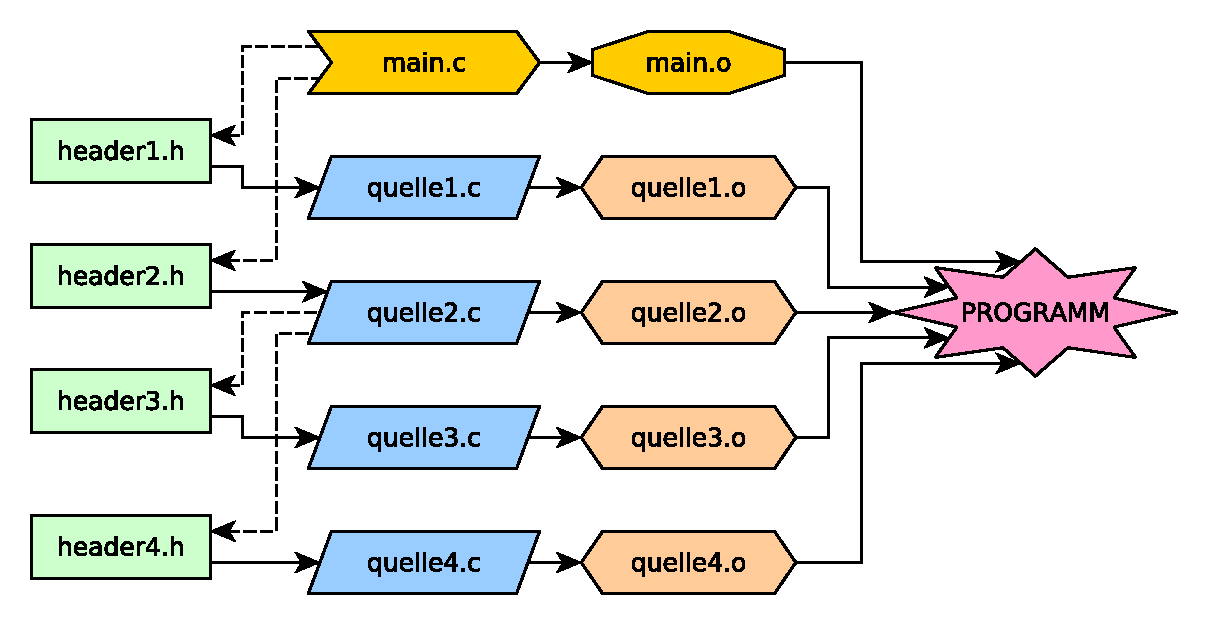
\includegraphics[width=\textwidth]{graphics/abhaengigkeiten}
  \caption{\label{fig:abhaengigkeiten} Struktur eines Programms mit vier Header- und fünf Quelltextdateien.}
\end{figure}

Das Übersetzen kann mithilfe eines \emph{Makefiles} einfacher, schneller und weniger anfällig auf Bedienungsfehler gemacht werden.
Ein Makefile ist eine Datei, welche bestimmte Regeln zum Übersetzen eines Programms beschreibt.
Die Struktur ist dabei relativ offen, da es sich eigentlich nur um eine Beschreibung von Abhängigkeiten und Regeln zur Erfüllung dieser Abhängigkeiten handelt.
Diese Abhängigkeiten werden mit dem Programm \texttt{make} Schritt für Schritt abgearbeitet, bis alle zum Verlinken des Programms notwendigen Teile zur Verfügung stehen.

Ein einfaches Makefile könnte wie folgt aussehen
\begin{lstlisting}
  regel: abhaengigkeit1 abhaengigkeit2 abhaengigkeit3
          kommando1
          kommando2
\end{lstlisting}

\endinput

